\subsection{Comparación de algoritmos}

En esta sección, comparamos varios algoritmos con respecto a nuestras métricas de interés: Accuracy, Precision, Recall y F1 Score (R2). Los algoritmos considerados se dividen en:

% -----------

\subsubsection{Comparacion y Analisis de Modelos de Clasificación}

\begin{itemize}
    \item DecisionTreeClassifier
    \item LogisticRegression
    \item RandomForestClassifier
    \item XGBClassifier
\end{itemize}

Para estos modelos, se utilizará la variable objetivo \say{aprobado}, la técnica \say{Stratified K-Fold Cross-Validation}, ajustaremos el mejor modelo en los datos de entrenamiento y realizaremos predicciones utilizando el mejor modelo.

La mejor configuración para los modelos de clasificación se muestra en el siguiente codigo: \ref{lst:config_clasificacion}:


\begin{lstlisting}[language=Python, caption=Definicion de los Modelos de Clasificación,label=lst:config_clasificacion]
    # Definir los modelos de Clasificacion
    models_clasificacion = [
        DecisionTreeClassifier(
            min_samples_split=10,
            min_samples_leaf=5,
        ),
        LogisticRegression(penalty="l2", C=1.0, solver="lbfgs", max_iter=150),
        RandomForestClassifier(
            max_depth=10,
            min_samples_split=10,
            min_samples_leaf=5,
            random_state=1502,
            n_estimators=500,
        ),
        XGBClassifier(learning_rate=0.1, max_depth=10, n_estimators=150, subsample=1.0),
    ]
\end{lstlisting}

% -----------

\subsubsection{Determinación de Características Clave y Variable Objetivo para Modelos de Clasificación}

En el siguiente fragmento de código, se lleva a cabo el proceso de selección de características relevantes para los modelos de clasificación. La variable objetivo, denominada aprobado, indica si un estudiante ha aprobado o no. Las características seleccionadas, representadas por X, incluyen diversos indicadores y hitos del estudiante, como hito1, hito2, y eventos específicos e0 a e52. Estas características se extraen del dataframe df y se utilizarán para entrenar y evaluar los modelos de clasificación.

\begin{lstlisting}[language=Python, caption=Selección de características y variable objetivo, label=lst:seleccion_caracteristicas]
y = df["aprobado"]
X = df[
['hito1', 'hito2', 'exitosos', 'fallidos','e0', 'e1', 'e2', 'e3', 'e4', 'e5', 'e6', 'e7', 'e8', 'e9', 'e10', 'e11', 'e12', 'e13', 'e14', 'e15', 'e16', 'e17', 'e18', 'e19', 'e20', 'e21', 'e22', 'e23', 'e24', 'e25', 'e26', 'e27', 'e28', 'e29', 'e30', 'e31', 'e32', 'e33', 'e34', 'e35', 'e36', 'e37', 'e38', 'e39', 'e40', 'e41', 'e42', 'e43', 'e44', 'e45', 'e46', 'e47', 'e48', 'e49', 'e50', 'e51', 'e52']
]
\end{lstlisting}

% -----------

\subsubsection{Validación Cruzada Estratificada y Ajuste de Modelos de Clasificación}

En el siguiente fragmento de código, se establece un proceso de validación cruzada estratificada para evaluar varios modelos de clasificación. Primero, definimos las métricas de interés: precisión, exhaustividad, exactitud y la puntuación F1. Luego, aplicamos la técnica de Stratified K-Fold Cross-Validation para garantizar que cada pliegue sea una buena representación del conjunto de datos completo. A continuación, entrenamos cada modelo y evaluamos su rendimiento utilizando las métricas definidas. Finalmente, identificamos y mostramos el modelo con el mejor rendimiento promedio.

\begin{lstlisting}[language=Python, caption=Aplicación de Stratified K-Fold y entrenamiento de modelos, label=lst:stratified_kfold]
    # Definir las métricas
    metrics = ["accuracy", "precision", "recall", "f1"]

    # Realizar Stratified K-Fold Cross-Validation en los datos de entrenamiento y obtener las métricas para cada modelo
    results_train = (
        {}
    )  # Diccionario para almacenar los resultados de entrenamiento de cada modelo

    for model in models_clasificacion:
        model_name = model.__class__.__name__

        cv = StratifiedKFold(n_splits=10, shuffle=True, random_state=1502)
        # Dividir los datos en conjuntos de entrenamiento y prueba
        X_train, X_test, y_train, y_test = train_test_split(
            X, y, test_size=0.2, random_state=1502
        )

        model.fit(X_train, y_train)  # Ajustar el modelo en los datos de entrenamiento
        model_results = (
            {}
        )  # Diccionario para almacenar los resultados de las métricas para el modelo actual

        # Calcular las métricas utilizando validación cruzada
        for metric in metrics:
            scores = cross_val_score(model, X_train, y_train, cv=cv, scoring=metric)
            model_results[metric] = scores

        results_train[
            model_name
        ] = model_results  # Almacenar los resultados del modelo en el diccionario

    best_model = None
    best_score = 0.0

    # Encontrar el mejor modelo basado en la media de las métricas
    for model_name, model_result in results_train.items():
        mean_scores = [np.mean(model_result[metric]) for metric in metrics]
        mean_score = np.mean(mean_scores)

        if mean_score > best_score:
            best_score = mean_score
            best_model = model_name

    # Imprimir el mejor modelo y su puntuación
    print("El mejor modelo en la validación fue:", best_model, best_score)
\end{lstlisting}

% -----------

\subsubsection{Resultados de la Validación Cruzada Estratificada}

Después de aplicar la validación cruzada estratificada y entrenar los modelos de clasificación, se evaluaron sus rendimientos utilizando varias métricas. El modelo que demostró tener el mejor rendimiento promedio fue el RandomForestClassifier, con una puntuación de 0.6433 (redondeado a cuatro decimales). Esta puntuación se calculó como el promedio de las métricas de precisión, exhaustividad, exactitud y la puntuación F1.

Con estos resultados, se destaca la eficacia del modelo de clasificación basado en bosques aleatorios para este conjunto de datos en particular, lo que sugiere que puede ser una opción adecuada para futuras predicciones o análisis relacionados.

\begin{lstlisting}[language=Python, caption=Resultado Mejor modelo en la Validacion de Clasificación, label=lst:rest_bestModelClasification]
    El mejor modelo en la validación fue: RandomForestClassifier 0.6432621955500205
    \end{lstlisting}



% -----------

\subsubsection{Predicciones con el Mejor Modelo en el Conjunto de Prueba}

En el siguiente fragmento de código, buscamos el objeto correspondiente al mejor modelo identificado previamente, en este caso, el RandomForestClassifier. Una vez encontrado, ajustamos este modelo utilizando el conjunto de entrenamiento y luego realizamos predicciones sobre el conjunto de prueba. Posteriormente, calculamos métricas clave, como el Mean Squared Error (MSE) y el R2 Score, para evaluar el rendimiento del modelo en el conjunto de prueba.

\begin{lstlisting}[language=Python, caption=Predicciones y evaluación del mejor modelo, label=lst:prediccion_mejor_modelo]
    best_model_search = None

    # Buscar el objeto del mejor modelo en la lista de modelos
    for model in models_clasificacion:
        if model.__class__.__name__ == best_model:
            best_model_search = model
            break
    
    best_model_search.fit(
        X_train, y_train
    )  # Ajustar el mejor modelo en los datos de entrenamiento
    y_pred = best_model_search.predict(
        X_test
    )  # Realizar predicciones utilizando el mejor modelo
    
    # Calcular y mostrar los resultados obtenidos del mejor modelo
    mse = mean_squared_error(y_test, y_pred)  # Calcular el Mean Squared Error
    r2 = r2_score(y_test, y_pred)  # Calcular el R2 Score
    
    print("Resultados del mejor modelo:", best_model, "en el conjunto de prueba:")
    print("Mean Squared Error:", mse)
    print("R2 Score:", r2)
    \end{lstlisting}

Después de realizar las predicciones con el RandomForestClassifier en el conjunto de prueba, obtuvimos los siguientes resultados:

Mean Squared Error (MSE): 0.3631 (redondeado a cuatro decimales)
R2 Score: 0.4532 (redondeado a cuatro decimales)

Estos resultados proporcionan una medida cuantitativa del rendimiento del modelo en el conjunto de prueba. Es importante notar que un R2 Score negativo indica que el modelo no es adecuado para predecir la variable objetivo en este conjunto de datos, y puede ser menos preciso que un modelo simple que siempre predice el valor medio.

% ------------

\subsubsection{Comparación Gráfica de Métricas de Rendimiento en Modelos de Clasificación (Conjunto de Entrenamiento)}

A continuación, se presentan los resultados obtenidos para el conjunto de entrenamiento. La Figura \ref{fig:metricas_clasificacion} ilustra las métricas de rendimiento de diversos modelos de clasificación evaluados.

\begin{figure}[H]
    \centering
    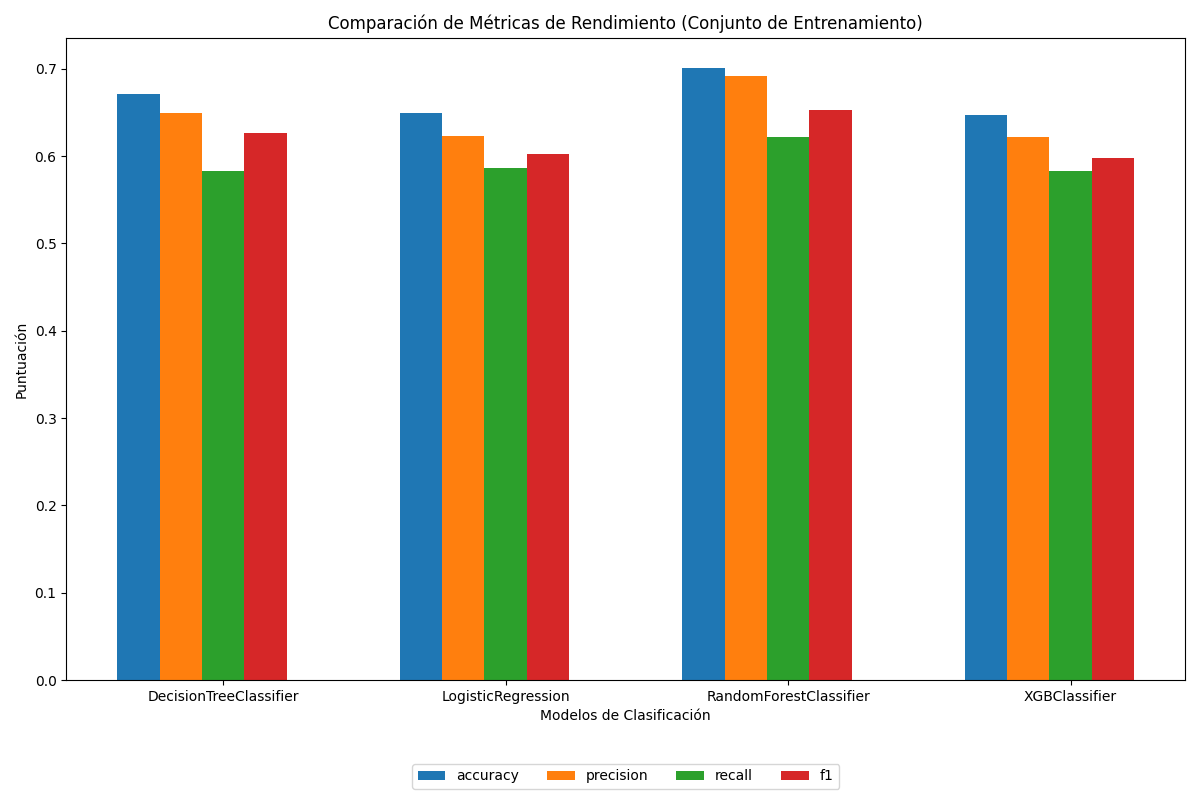
\includegraphics[width=1\textwidth]{img/compara_algoritmos/metricasEntreModelosClasificacion.png}
    \caption{Comparativa de métricas entre modelos de clasificación para el conjunto de entrenamiento.}
    \label{fig:metricas_clasificacion}
\end{figure}

La figura destaca que el modelo RandomForestClassifier sobresale en comparación con los otros modelos en todas las métricas evaluadas. En particular, este modelo logra un F1 Score de 62.53\%, un recall de 58.90\%, una precisión de 67.61\% y una exactitud de 66.54\%.

Para una visión más detallada y estructurada de estos resultados, se presenta la siguiente tabla:

\begin{table}[H]
    \centering
    \caption{Comparación de Métricas de Rendimiento para Modelos de Clasificación}
    \begin{tabular}{lcccc}
        \toprule
        \textbf{Modelo} & \textbf{Accuracy} & \textbf{Precision} & \textbf{Recall} & \textbf{F1} \\
        \midrule
        DecisionTreeClassifier & 0.6409 & 0.6300 & 0.5194 & 0.5708 \\
        LogisticRegression & 0.6617 & 0.6446 & 0.5792 & 0.6069 \\
        RandomForestClassifier & 0.6826 & 0.6761 & 0.5890 & 0.6253 \\
        XGBClassifier & 0.6186 & 0.5865 & 0.5262 & 0.5534 \\
        \bottomrule
    \end{tabular}
    \label{tab:performance_metrics}
\end{table}

Para el conjunto de prueba, los resultados se muestran en la Figura \ref{fig:metricas_clasificacion_bestModel}.

\begin{figure}[H]
    \centering
    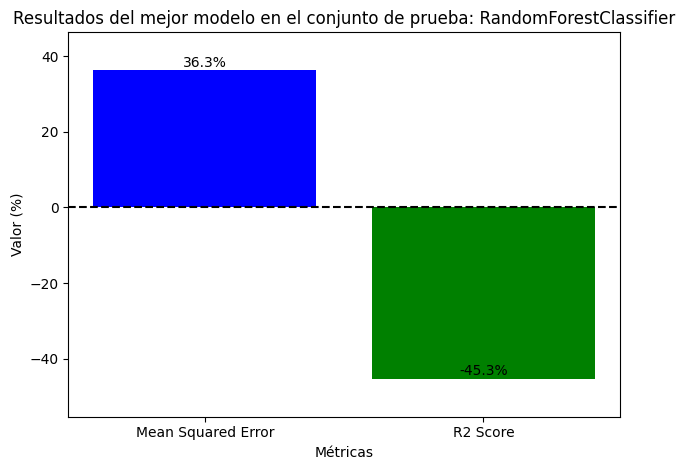
\includegraphics[width=0.8\textwidth]{img/compara_algoritmos/metricasBestModelRandomForesClassifier.png}
    \caption{Métricas del mejor modelo de clasificación en el conjunto de prueba.}
    \label{fig:metricas_clasificacion_bestModel}
\end{figure}

Las métricas cuantitativas para el conjunto de prueba son:

\begin{itemize}
    \item Mean Squared Error: 36.3\%
    \item R2 Score: -45.3\%
\end{itemize}

Con base en los resultados obtenidos, se concluye que el modelo RandomForestClassifier es el más adecuado para abordar este problema de clasificación. En la validación, este modelo demostró ser el mejor, con una puntuación del 62.53\%.

% -----------

\subsubsection{Comparacion y Analisis de Modelos de Regresión}

La regresión es una técnica estadística que permite modelar y analizar las relaciones entre una variable dependiente y una o más variables independientes.

\begin{itemize}
    \item LinearRegression
    \item DecisionTreeRegressor
    \item KNeighborsRegressor
\end{itemize}

Para estos modelos, se utilizará la variable objetivo \say{sol1}, la técnica \say{K-Fold Cross-Validation}, ajustaremos el mejor modelo en los datos de entrenamiento y realizaremos predicciones utilizando el mejor modelo.

La mejor configuración para los modelos de regresión se en el siguiente codigo: \ref{lst:config_regresion}:

\begin{lstlisting}[language=Python, caption=Configuración de los modelos de regresión, label=lst:config_regresion]
# Definir los modelos de regresión
models_regresion = [
    LinearRegression(positive=True, fit_intercept=True),
    DecisionTreeRegressor(
        min_samples_split=5,
        min_samples_leaf=3,
    ),
    KNeighborsRegressor(n_neighbors=8),
]
    \end{lstlisting}

% -----------

\subsubsection{Selección de Características y Variable Objetivo}
Antes de entrenar los modelos, es crucial seleccionar las características que se utilizarán para la predicción y definir la variable objetivo. Esta selección garantiza que los modelos se entrenen con la información más relevante.

\begin{lstlisting}[language=Python, caption=Seleccion de caracteristica y variable objetivo, label=lst:config_varObjetivoCaracteristicas]
# Selección de características y variable objetivo para los modelos de Regresion.
y = df["sol1"]
X = df[
['hito1', 'hito2', 'exitosos', 'fallidos','e0', 'e1', 'e2', 'e3', 'e4', 'e5', 'e6', 'e7', 'e8', 'e9', 'e10', 'e11', 'e12', 'e13', 'e14', 'e15', 'e16', 'e17', 'e18', 'e19', 'e20', 'e21', 'e22', 'e23', 'e24', 'e25', 'e26', 'e27', 'e28', 'e29', 'e30', 'e31', 'e32', 'e33', 'e34', 'e35', 'e36', 'e37', 'e38', 'e39', 'e40', 'e41', 'e42', 'e43', 'e44', 'e45', 'e46', 'e47', 'e48', 'e49', 'e50', 'e51', 'e52']
]
\end{lstlisting}


% -----------
\subsubsection{Validación Cruzada y Entrenamiento}
La validación cruzada es una técnica que permite evaluar la capacidad de generalización de los modelos. En este estudio, se utiliza K-Fold Cross-Validation para entrenar y validar los modelos de regresión en diferentes subconjuntos del conjunto de datos.

\begin{lstlisting}[language=Python, caption=Configuraicones previas antes de la evaluación, label=lst:config_preEval]
# Listas para almacenar los resultados de cada modelo
mse_scores = []
mae_scores = []
r2_scores = []

best_model = None
best_mse = np.inf
best_mae = np.inf
best_r2 = -np.inf

# Colores para los modelos de regresión
colors = ["blue", "green", "red"]
    \end{lstlisting}

% -----------
\paragraph{Evaluación de Modelos de Regresión}
Una vez entrenados, es esencial evaluar el rendimiento de cada modelo. Esta evaluación se basa en métricas específicas que reflejan la precisión y eficacia de los modelos en la predicción de la variable objetivo.

\begin{lstlisting}[language=Python, caption=Codigo de evaluacion de modelos, label=lst:cod_Eval]
# Iterar sobre cada modelo de regresión
for i, model in enumerate(models_regresion):
    # Realizar k-fold cross-validation
    kf = KFold(n_splits=10, shuffle=True, random_state=1502)
    mse_cv_scores = []
    mae_cv_scores = []
    r2_cv_scores = []
    
    for train_index, test_index in kf.split(X):
        # Train-test split para cada fold
        X_train, X_test = X.iloc[train_index], X.iloc[test_index]
        y_train, y_test = y.iloc[train_index], y.iloc[test_index]
        
        # Entrenar el modelo
        model.fit(X_train, y_train)
        
        # Realizar predicciones en el conjunto de prueba
        y_pred = model.predict(X_test)
        
        # Calcular las métricas de evaluación
        mse = mean_squared_error(y_test, y_pred)
        mae = mean_absolute_error(y_test, y_pred)
        r2 = r2_score(y_test, y_pred)
        
        # Almacenar las métricas de evaluación para cada fold
        mse_cv_scores.append(mse)
        mae_cv_scores.append(mae)
        r2_cv_scores.append(r2)
        
    # Calcular la media de las métricas de evaluación para el modelo actual
    avg_mse = np.mean(mse_cv_scores)
    avg_mae = np.mean(mae_cv_scores)
    avg_r2 = np.mean(r2_cv_scores)
    
    # Almacenar las métricas de evaluación para el modelo actual
    mse_scores.append(avg_mse)
    mae_scores.append(avg_mae)
    r2_scores.append(avg_r2)
    
    # Verificar si el modelo actual es el mejor hasta ahora
    if avg_mse < best_mse:
        best_model = model
        best_mse = avg_mse
        best_mae = avg_mae
        best_r2 = avg_r2
    \end{lstlisting}

% -----------

\subsubsection{Resultados y Comparación}
Tras la evaluación, se presentan los resultados obtenidos de cada modelo. Estos resultados permiten identificar qué modelo tiene el mejor rendimiento en términos de precisión y eficacia.

Los resultados obtenidos se presentan en la Figura \ref{fig:metricas_regresion}:

\begin{figure}[H]
    \centering
    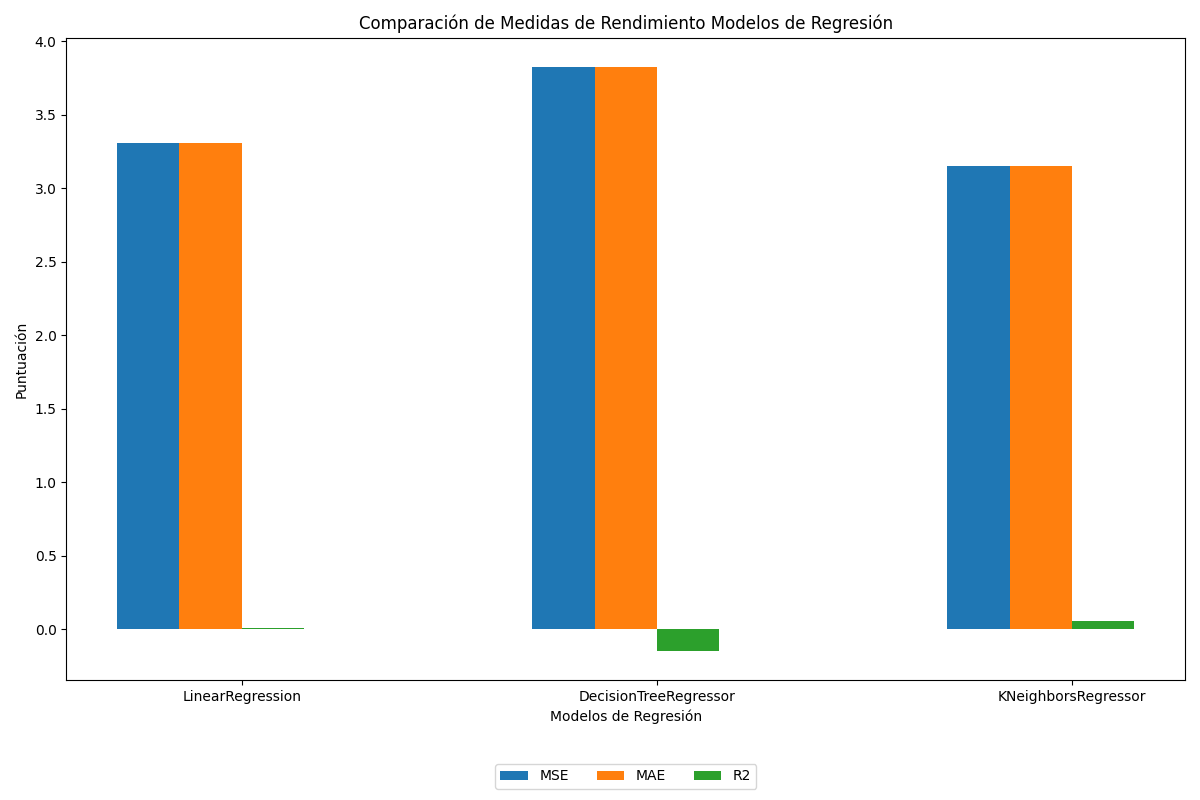
\includegraphics[width=1\textwidth]{img/compara_algoritmos/metricasEntreModelosRegresion.png}
    \caption{Métricas entre modelos de regresión conjunto de entrenamiento}
    \label{fig:metricas_regresion}
\end{figure}

Se observa que el modelo LinearRegression en su conjunto de entrenamiento presenta el comportamiento mas normal utilizando la validacion k-fold cross-validation para variables cuantitativas.

Los resultados sobre el conjunto de prueba se presentan en la figura \ref{fig:metricas_regresion_bestModel}

\begin{figure}[H]
    \centering
    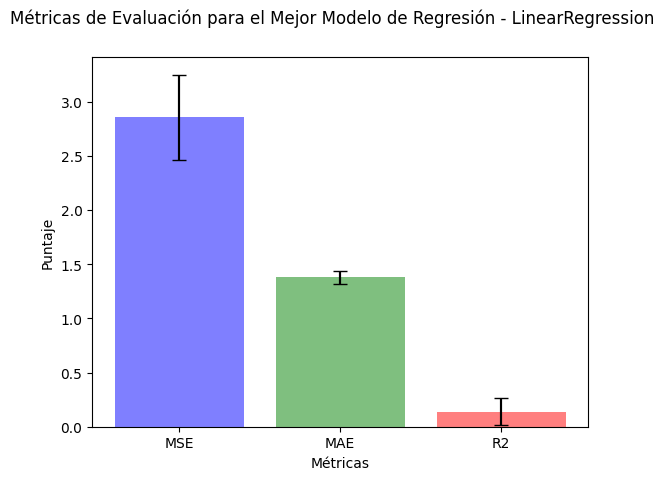
\includegraphics[width=0.7\textwidth]{img/compara_algoritmos/metricasBestModelLinearRegression.png}
    \caption{Métricas Best Model}
    \label{fig:metricas_regresion_bestModel}
\end{figure}

Se observa que el modelo LinearRegression es el mejor modelo de regresión, con un MSE del 3.6\% y un MAE del 1.6\%, valores inferiores a los de los otros modelos evaluados. Además, el modelo LinearRegression presenta un R2 más cercano a 1, con un aumento del 0.1\% en comparación con los demás modelos.

En base en los resultados obtenidos, se puede concluir que el modelo LinearRegression es el más adecuado para problemas de regresion con variable cuantitativas.

\begin{itemize}
    \item El mejor modelo en la validación fue: LinearRegression 14.1\%
\end{itemize}

Resultados del mejor modelo en el conjunto de prueba:

\begin{itemize}
    \item MSE: 3.6.\%
    \item MAE: 1.6\%
    \item R2: 0.1\%
\end{itemize}

% -----------

\subsubsection{Conclusión}

En conclusión, se realizó una comparación exhaustiva de diferentes algoritmos de modelos predictivos para determinar cuál es el más adecuado en términos de origen de datos. Después de analizar y comparar varios algoritmos, se llegó a la conclusión de que el modelo RandomForestClassifier se destaca como el enfoque más efectivo para el origen de datos en cuestión, mientras que el modelo LinearRegression es el más adecuado para análisis de regresión.